\begin{figure*}[hbtp]
  \centering
  % \includegraphics[width=0.44\linewidth]{out/5050-error-key.pdf}
  \subfigure[Overall result]{
    \label{fig:5050-error--mean}
    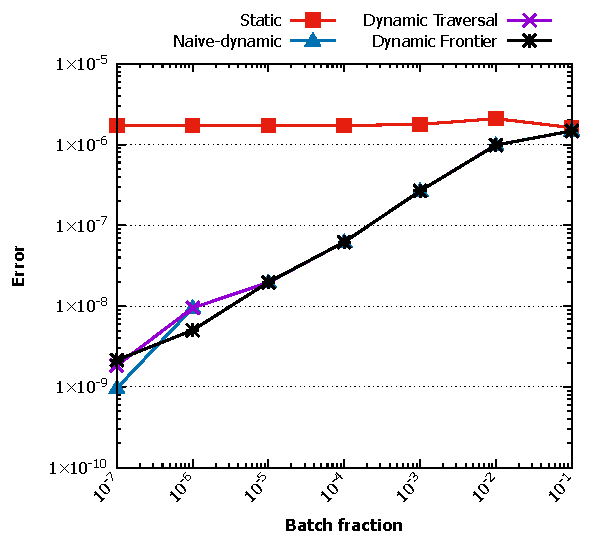
\includegraphics[width=0.38\linewidth]{out/5050-error-mean.pdf}
  }
  \subfigure[Results on each graph]{
    \label{fig:5050-error--all}
    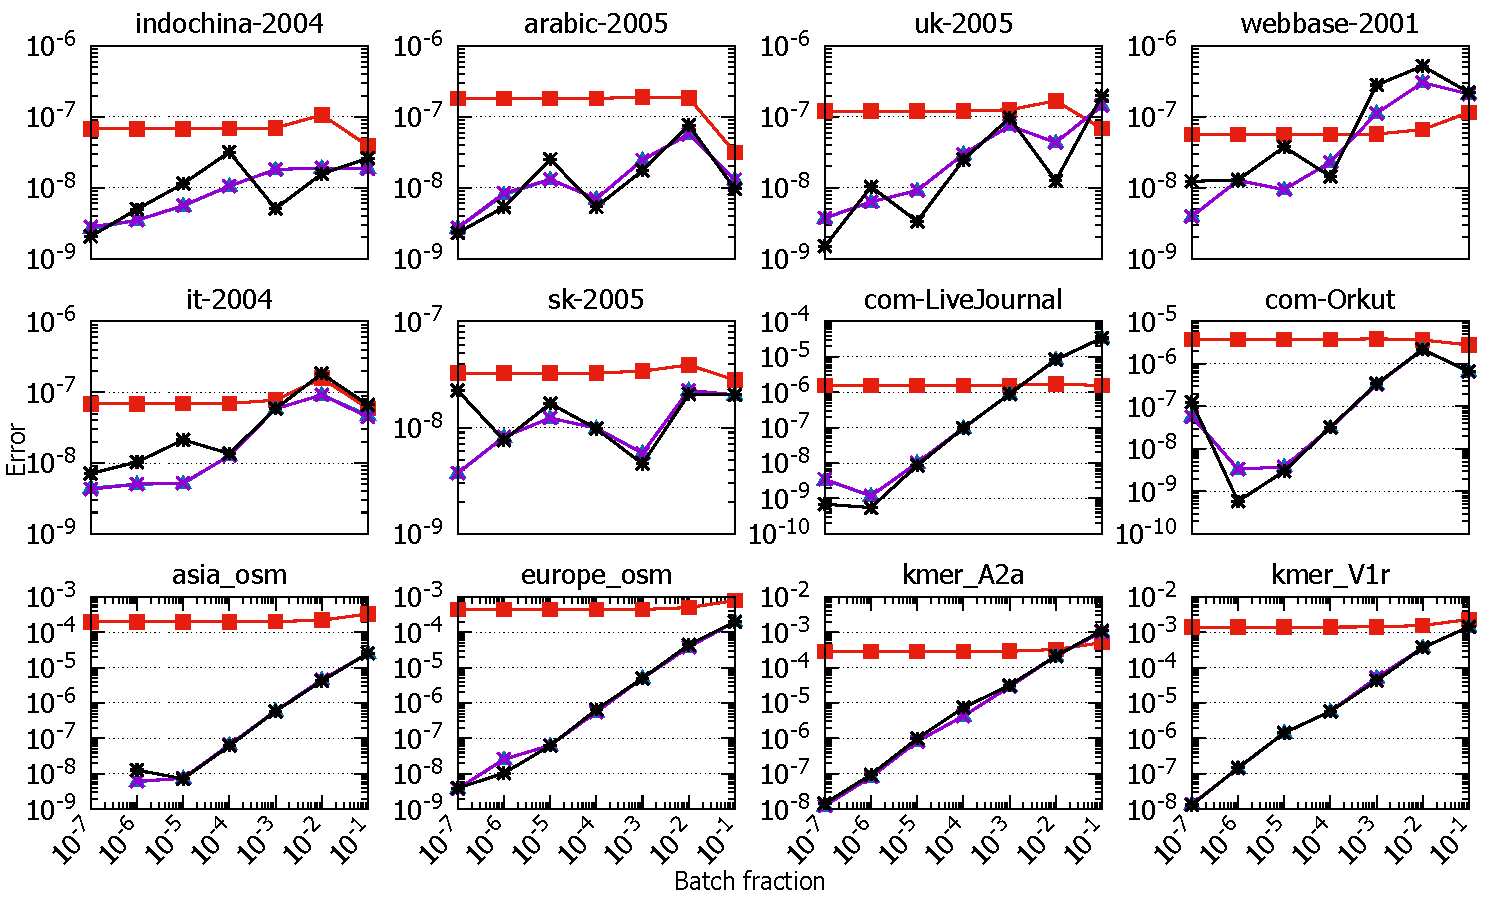
\includegraphics[width=0.58\linewidth]{out/5050-error-all.pdf}
  } \\[-1ex]
  \caption{Error comparison of \textit{Static}, \textit{Naive-dynamic}, \textit{Dynamic Traversal}, and \textit{Dynamic Frontier} PageRank with respect to a Reference Static PageRank (with a tolerance $\tau$ of $10^{-100}$ and limited to $500$ iterations), using $L1$-norm. Batch updates range from $10^{-7} |E|$ to $0.1 |E|$ (logarithmic scale), consisting of $80\%$ edge insertions and $20\%$ edge deletions to simulate realistic dynamic graph updates. The right figure depicts the error for each approach in relation to each graph, while the left figure showcases overall errors using geometric mean for consistent scaling across graphs.}
  \label{fig:5050-error}
\end{figure*}
